\documentclass[en]{../../../eplsummary}
\usepackage{framed}
\usepackage{placeins}
\usepackage{listings}
\usepackage{color}

\definecolor{dkgreen}{rgb}{0,0.6,0}
\definecolor{gray}{rgb}{0.5,0.5,0.5}
\definecolor{mauve}{rgb}{0.58,0,0.82}

\lstset{frame=tb,
  language=Java,
  aboveskip=3mm,
  belowskip=3mm,
  showstringspaces=false,
  columns=flexible,
  basicstyle={\small\ttfamily},
  numbers=none,
  numberstyle=\tiny\color{gray},
  keywordstyle=\color{blue},
  commentstyle=\color{dkgreen},
  stringstyle=\color{mauve},
  breaklines=true,
  breakatwhitespace=true,
  tabsize=3
}

\graphicspath{{res/}}

\hypertitle{algo-INGI2266}{7}{INGI}{2266}
{Houtain Nicolas}
{de Vogelaere Cyril}
{Pierre Schaus}

\section{Dynamic programing}

\subsection{Definition}

\textbf{Dynamic programming} is a method by recurrence in order to solve complex problem.
\begin{itemize}
    \item breaking it down into a collection of simpler subproblems
    \item solving each of those subproblems just once, and storing their solutions in memory
    \item[$\rightarrow$] Next time the same subproblem occurs, instead of 
recomputing its solution, only looks up to the previously computed solution.
Thereby \textbf{saving computation time at the expense of storage space}.
\end{itemize}

\subsection{Solving the knapsack problem with DP}

\subsubsection{The knapsack problem}
\begin{itemize}
    \item A set of item $I$
    \item for each item $i \in I$ is associated a value $v_i$ and a weight $w_i$.

    \item[Goals] 
        \begin{tabular}{m{3cm}m{12cm}}
            $\sum_{i \in I} v_i x_i$: & Maximize the value of selected items\\
            $\sum_{i \in I} w_i x_i \le C$ & Under constraint that the total
            capacity cannot exceed a given maximal capacity $C$ \\ 
            $x_i \in \{0,1\}$ & And an item cannot be partially selected \\
        \end{tabular}
\end{itemize}

Note that Knapsack is an NP-Complete problem as it can be used
to find a solution to the subset-sum problem, which is NP-complete.

\paragraph{Subset-sum problem}

Given a set of natural number and a capacity K. 
Find a subset S such that :
$$\sum_{i \in S} c_i = K$$


\subsubsection{Solutions}
\begin{itemize}
    \item \textbf{DP for knapsack in 0(Cn)}.

        Refer to the optimal objective of the problem with capacity $k$ and
        items \{1,…,j\} $\in$ I as $O(k,j)$. We can easily notice that :

        \begin{itemize}
            \item $O(k,0) = 0 \text{\footnotemark}$
            \item $ O(k,j) = \begin{cases} 
                    max(O(k,j-1) , vj +O(k-wj,j-1))\text{\footnotemark} & if \quad w_j \leq k \\
                    O(k,j-1) & otherwise
                \end{cases}$
        \end{itemize}
        \footnotetext{As their are no elements to choose from}
        \footnotetext{Bellman's equations}


        \begin{lstlisting}[caption=Knapsack DP]
val items = Array((1,1),(6,2),(18,5),(22,6),(28,7)) // (value,weight)
val C = 11
def O(j: Int, k: Int): Int = {
    if (j < 0) 0
    else {
        val (vj,wj) = items(j)
        if (wj > k) O(j-1,k)
        else O(j-1,k).max(vj + O(j-1,k-wj))
    }
}
println(O(items.size-1,C))
        \end{lstlisting}

        \begin{center}
    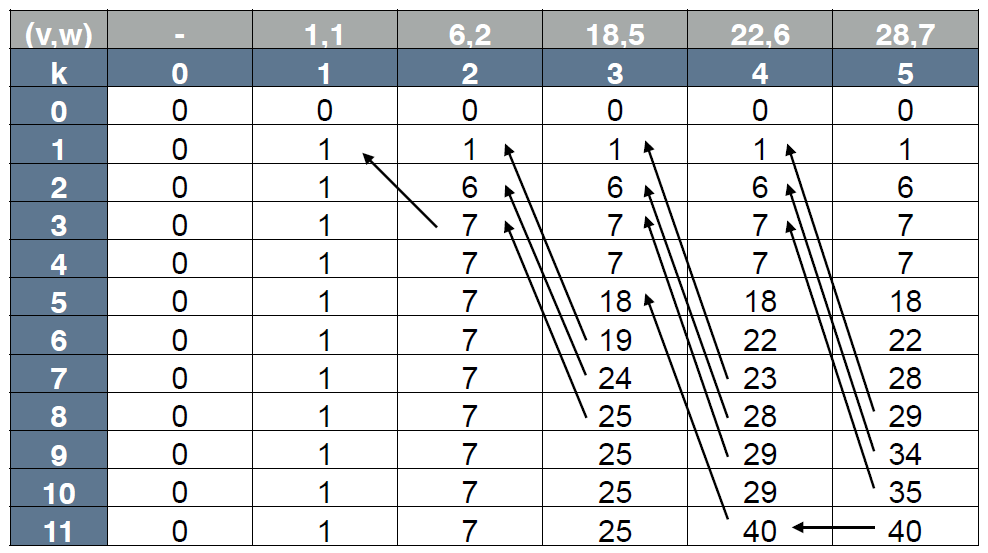
\includegraphics[width=7cm]{KnapsackDP.png}
        \end{center}

    \item \textbf{DP for knapsack in 0(Vn)}.

        Using a similar logic, it is also possible to define an algorithm which
        run in $\theta$(Vn) to compute knapsacks. Let $V = \sum_{i \in I} v_i$,
        we can redefine O(k,j) as O(w,j), the optimal weight using only items
        \{1,...,j\}. The equation will thus change as follow :

    \begin{itemize}
    \item $O(0,j) = O(w,0) = 0 \text{\footnotemark} $
    \item $ O(w,j) = \begin{cases}
                min(O(w,j-1), wi + O(w-v_j,j-1)) & if \quad v_j \leq p \\
                O(w,j-1) & otherwise
            \end{cases}$
        \end{itemize}
        \footnotetext{As $w_i > 0$ for all $i \in I$ and as we cannot have w > 0 with 
        an empty set.}
        \begin{center}
            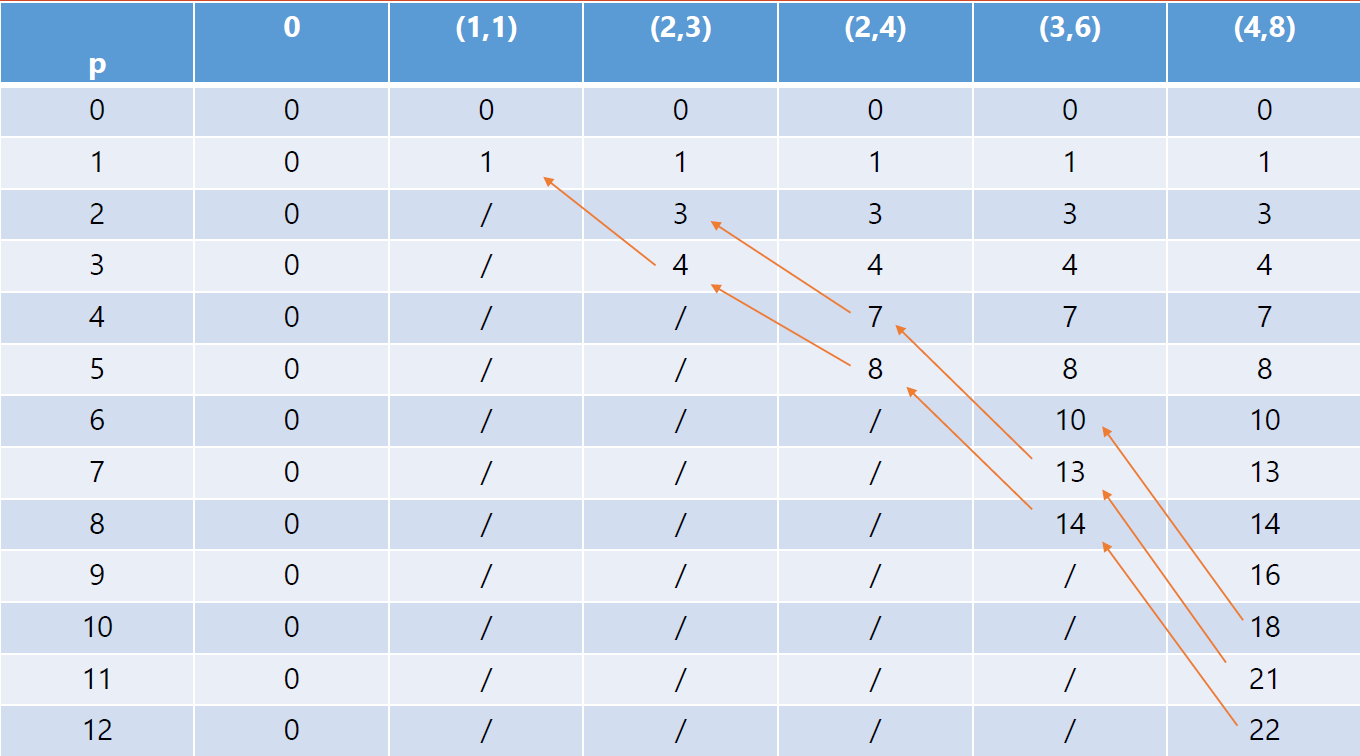
\includegraphics[width=7cm]{KnapsackDPAlgo2.png}
        \end{center}
\end{itemize}

\subsubsection{Cache usage}
\begin{tabular}{m{9cm}m{6cm}}
As explain, a cache is use in order to store computed value and avoid to recompute
it. In \textcolor{red}{red} we have the cells actually computed.
&
    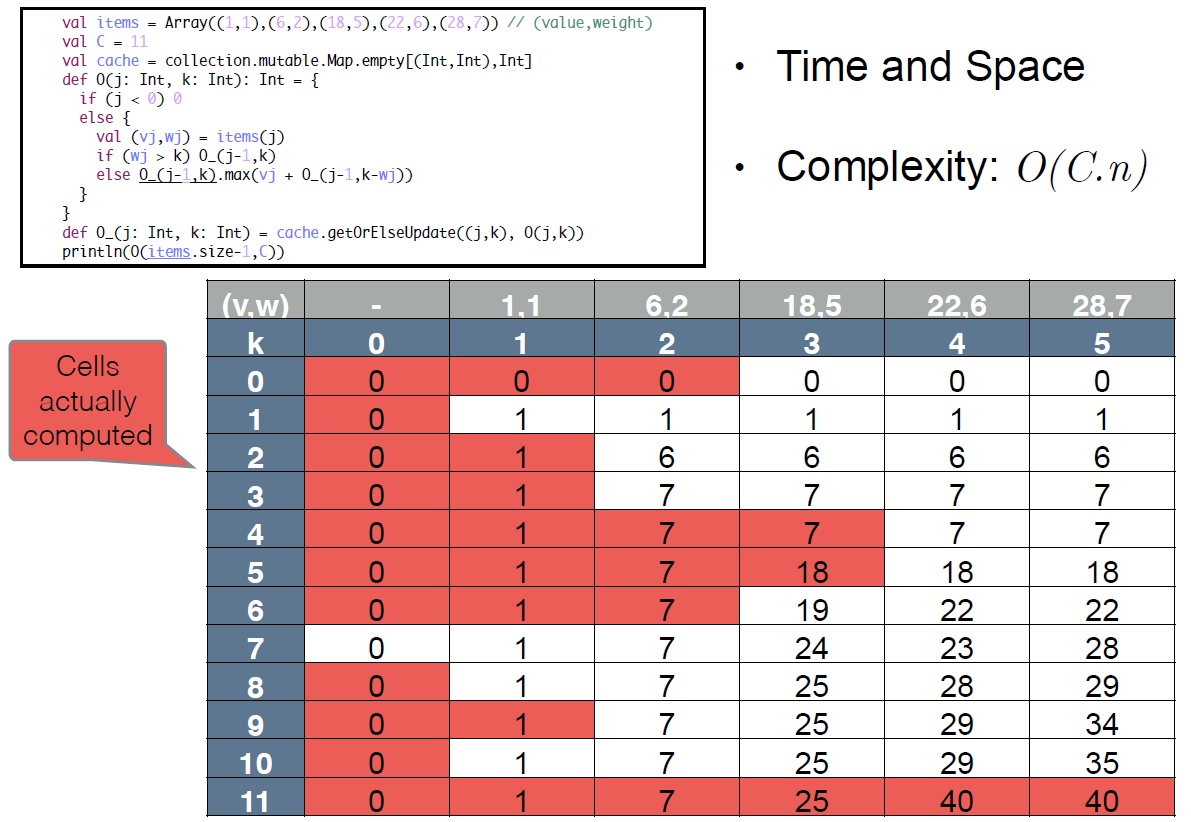
\includegraphics[width=6cm]{KnapsackDPAlgo1.png}
\end{tabular}


\subsubsection{Pseudo-polynomial}

DP is \textsc{pseudo-polynomial}, since it is exponential in the 
\textit{length of input} ($log(C)$) which is the number of bits required to
encode the input ($C$). The complexity is thus exponential relatively to the
input size. This algorithm is \textbf{weakly NP-Complete} or
\textbf{pseudo-polynomial}\footnote{a numeric algorithm runs in
pseudo-polynomial time if its running time is polynomial in the numeric value
of the input, but is exponential in the length of the input – the number of
bits required to represent it.} as it is roughly polynomial for small values of
C while computing larger value is much more expensive\footnote{Not all
    NP-Complete algorithm are pseudo polynomial ! Like the traveling salesman
problem (TSP), for example.}.


\subsection{Other examples of DP algorithms}

Before reading this section, please remember that all algorithm that can be
implemented via dynamic programming are not ipso-facto pseudo polynomial ! Any
algorithm can be expressed with dynamic programming as long as it can be separated in
sub problems.

\subsubsection{Edit distance}


TODO

\subsubsection{TSP}
 
TODO



\subsection{Exam}
I give you a problem (for instance the TSP, Knapsack)
\begin{itemize}
    \item  Design a greedy algorithm
    \item  Design a Dynamic Programming formulation
    \item  Design a relaxation and upper/lower bound
        procedure and embed it in a Branch and Bound
    \item  Justify advantages and disadvantages of each
    \item  Apply the three techniques to a small instance
        manually
\end{itemize}



\section{Branch and bound}

\subsection{Definition}

A \textbf{branch-and-bound} algorithm consists of a systematic enumeration of candidate solutions by means of state space search: the set of candidate solutions is thought of as forming a rooted tree with the full set at the root. The algorithm explores branches of this tree, which represent subsets of the solution set. Before enumerating the candidate solutions of a branch, the branch is checked against upper and lower estimated bounds on the optimal solution, and is discarded if it cannot produce a better solution than the best one found so far by the algorithm.

\subsection{Solving the knapsack problem with B\&B}

Given the following knapsack problem :

\begin{figure}[!ht]
    \centering
    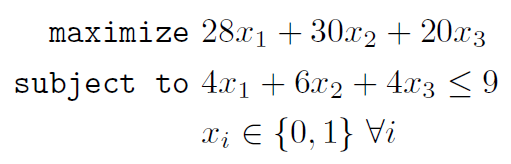
\includegraphics[width=0.4\linewidth]{KnapsackBBProblem.png}
    \label{fig:Knapsack_example}
\end{figure}
\FloatBarrier

We can choose to relax either of the constraint during the branch and bound procedure 
as to obtain a solution. The goal being to reduce the search space as much as possible
by calculating an upper bound as precise as possible.
Let us thus compare both options in the following sections.

\subsubsection{Capacity relaxation}

The first constraint that we can relax is the capacity constraint. The B\&B
calculation becomes fairly simple to implement as we only cut at tree branch when 
we have surpassed the capacity. The search space is thus reduced as such :

\begin{figure}[!ht]
    \centering
    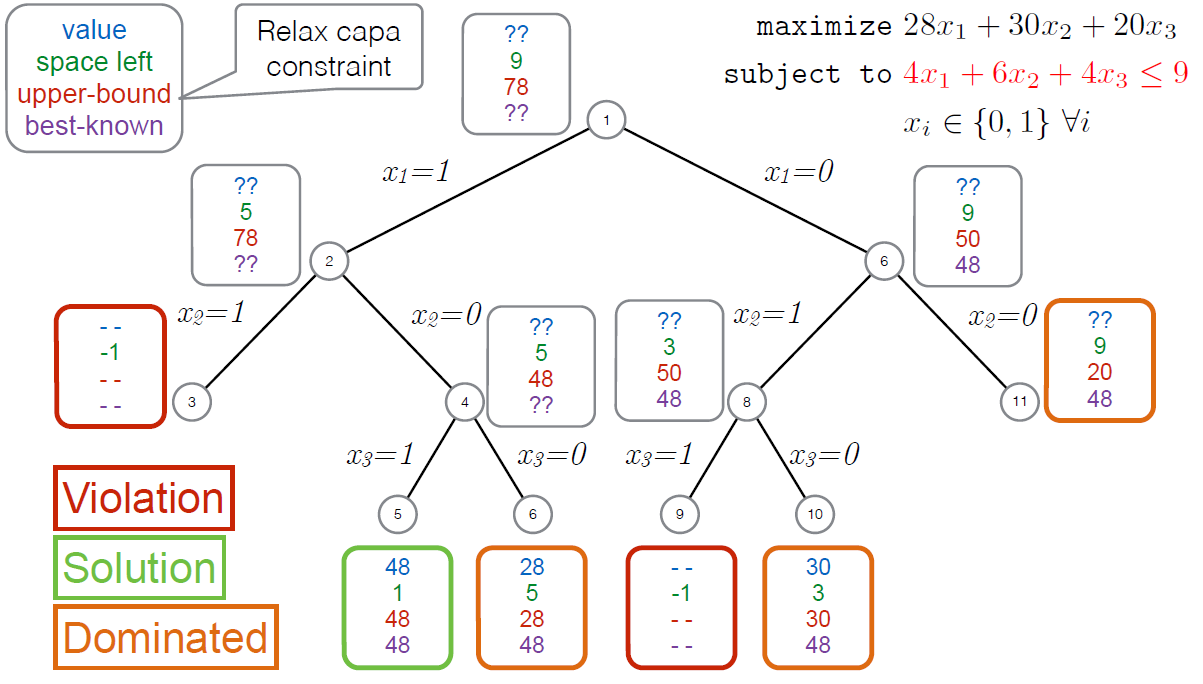
\includegraphics[width=\linewidth]{KnapsackBBCapaRelaxation.png}
    \label{fig:Knapsack_example}
\end{figure}
\FloatBarrier

Which, as you can see, is far from optimal as our upper bound are not close enough to their
real value.

\subsubsection{Linear relaxation}

This second relaxation is slightly harder to implement but yields better result, as 
the upper bound approximation is far better. Given a set sorted by ratio $v_i/w_i$,
the upper bound calculation procedure become as search for the first critical item j.
\newline

The first critical item j being the first item which cannot be fully added in our selection
due to capacity constraint. 

\begin{figure}[!ht]
    \centering
    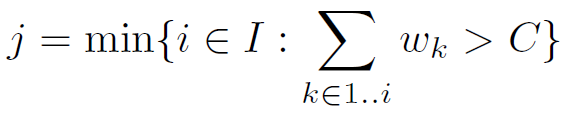
\includegraphics[width=0.4\linewidth]{KnapsackBBCriticalItem.png}
    \label{fig:Knapsack_example}
\end{figure}
\FloatBarrier

The upper bound can then be calculated as the sum of all item i < j plus as much of j
as we can squeeze in while respecting the capacity constraint.

\begin{figure}[!ht]
    \centering
    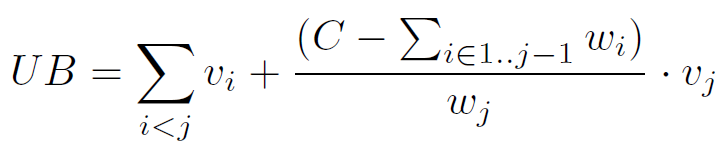
\includegraphics[width=0.5\linewidth]{KnapsackBBLinearRelaxationUB.png}
    \label{fig:Knapsack_example}
\end{figure}
\FloatBarrier

The search space is thus reduced as such :

\begin{figure}[!ht]
    \centering
    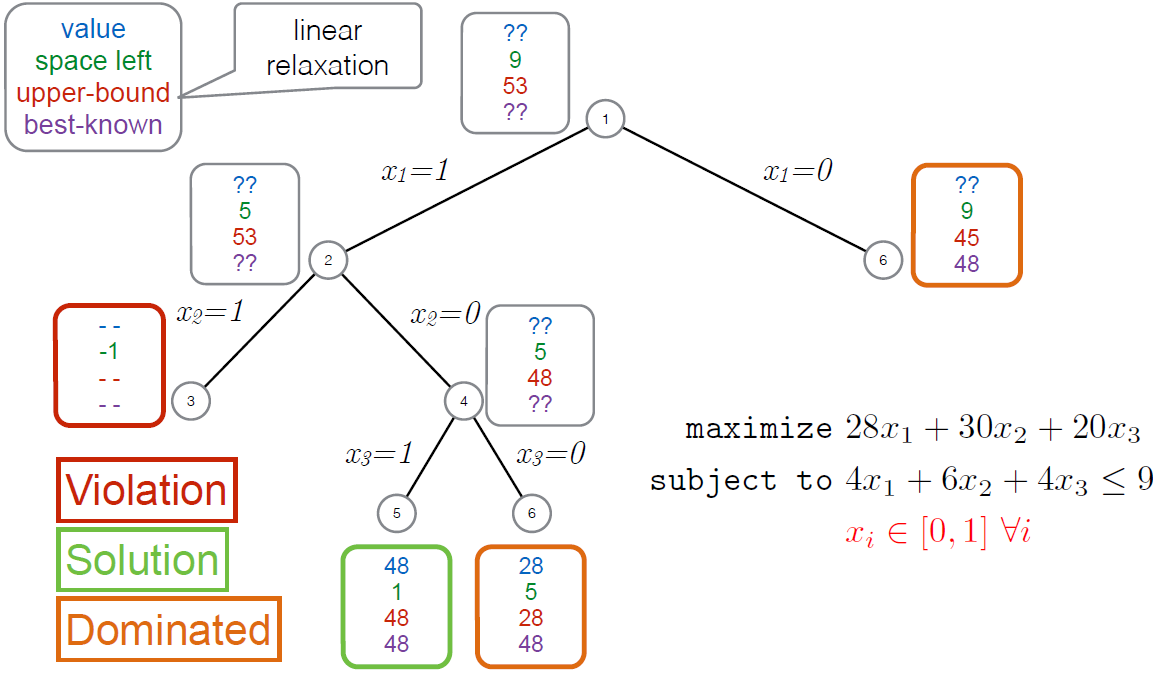
\includegraphics[width=\linewidth]{KnapsackBBLinearRelaxation.png}
    \label{fig:Knapsack_example}
\end{figure}
\FloatBarrier

As you can see, improving the precision of the upper-bound yields far better result. Take care however not to over/under estimate it (depending if you are on a maximisation or minimisation process) as it might prevent you to find the optimal solution.





\section{Search}
%TODO slides 3


\section{Lagrangian relaxation}
%TODO slides 4


\section{Network flow}
%TODO slides 5


\section{Greedy approximation}
%TODO slides 6


\section{Local search}
%TODO slides 7


\section{Constraint programming}
%TODO slides 8


\section{Local Neighbors Search}
%TODO slides 9


\section{Derivative free optimization}
%TODO slides 10


\section{Bi-objective}
%TODO slides 11




\end{document}
